\documentclass{beamer}
\usepackage[T1]{fontenc}
\usepackage{sansmathaccent}
\pdfmapfile{+sansmathaccent.map}
\usepackage{polski}
\usepackage[utf8]{inputenc}
\usepackage[polish]{babel}
\usepackage{caption}
\usepackage{pgfpages}
%\setbeameroption{show notes}
%\setbeameroption{show notes on second screen=right}
\mode<presentation>
{
	\usetheme{Warsaw}      % or try Darmstadt, Madrid, Warsaw, ...
	\usecolortheme{whale} % or try albatross, beaver, crane, ...
	\usefonttheme{default}  % or try serif, structurebold, ...
	\setbeamertemplate{headline}{}
	\setbeamertemplate{caption}[numbered]
} 

\title[Praca magisterska]{Rekomendacje artykułów opisujących produkty w serwisach e-commerce}
\author{Łukasz Dragan}
\institute{Informatyka spec. Metody sztucznej inteligencji, MiNI PW}
\date{07.12.2017}
\AtBeginSection[]{
	\begin{frame}
		\vfill
		\centering
		\begin{beamercolorbox}[sep=8pt,center,shadow=true,rounded=true]{title}
			\usebeamerfont{title}\insertsectionhead\par%
		\end{beamercolorbox}
		\vfill
	\end{frame}
}

\begin{document}
	
	\begin{frame}
		\titlepage
	\end{frame}
	\note{
		\begin{itemize}
			\item 
		\end{itemize}
		}
	\begin{frame}{Plan prezentacji}
	  \tableofcontents
	\end{frame}
	\note{
		\begin{itemize}
			\item po kolei co zamierzam powiedzieć
		\end{itemize}
	}
	\section{Opis problemu}
	
	\begin{frame}{Cel pracy}
		Czy metody semantycznej analizy tekstu mogą być alternatywą dla~dotychczas używanej przez~\emph{Allegro} metody generowania rekomendacji artykułów tekstowych?

	\end{frame}
		\note{
			\begin{itemize}
				\item nie znałem wcześniej tej tematyki
				\item realne biznesowe zastosowanie informatyki
				\item zaznajomiłem się z dziedziną, której wcześniej nie znałem
			\end{itemize}
		}

	
	\begin{frame}{allegro.pl}
		\begin{figure}
			\centering
			
\includegraphics[width=1\textwidth]{img/screen_allegro.png}
		\end{figure}
	\end{frame}
			\note{
				\begin{itemize}
					\item w Allegro prócz głóœnej funkcjonalności
					\item artykuły opisujące produkty
					\item zawiera listę artykułów podobnych, którą można uznać za rekomendacje
				\end{itemize}
			}
	\begin{frame}{allegro.pl cd}
		\begin{figure}
			\centering
			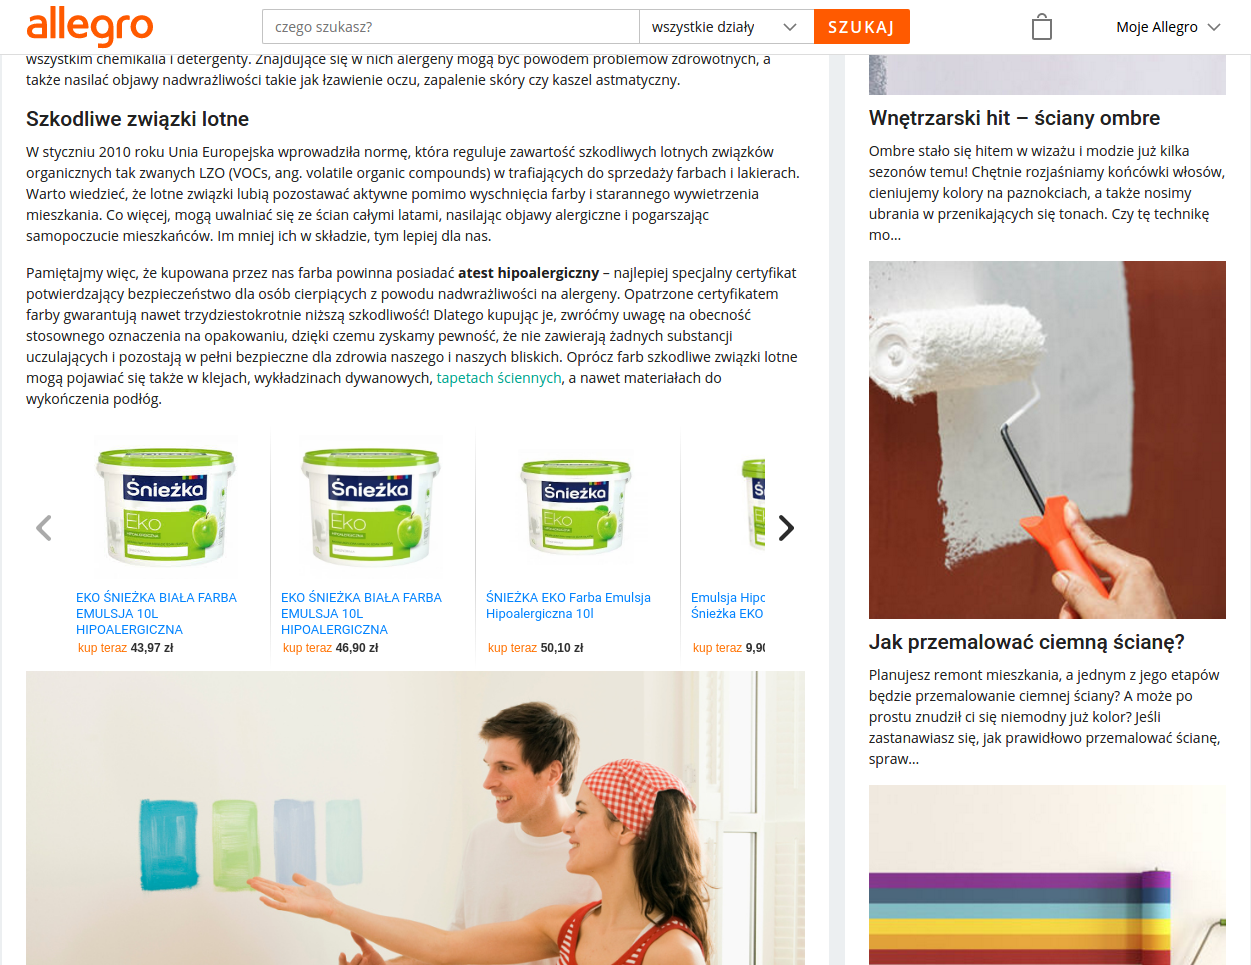
\includegraphics[width=1\textwidth]{img/screen_allegro_2.png}
		\end{figure}
	\end{frame}

	\section{Systemy rekomendacji}
	\note{
		Systemy wyszukiwania mają na~celu sugerowanie tego, co może się wydać użytkownikowi interesujące.
	}
	\begin{frame}{Systemy rekomenadacji}
		\begin{figure}
			\centering
			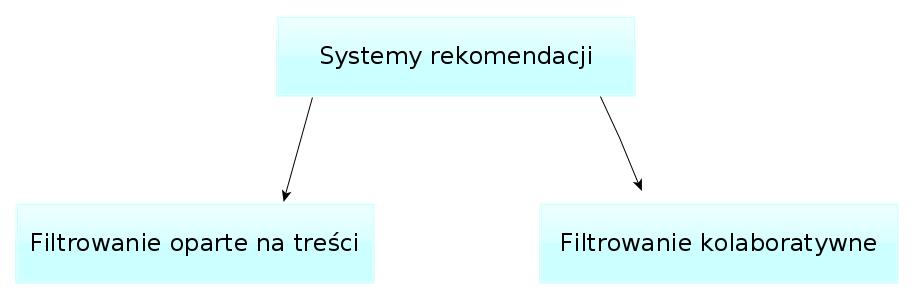
\includegraphics[width=1\textwidth]{img/recommender.png}
		\end{figure}
	\end{frame}
	\note{
		\begin{itemize}
			\item kolaboratywne generuje rekomendacje na podstawie aktywności użytkowników o podobnym profilu
			\item jest niezależne od dziedziny
			\item .
			\item oparte na treści generuje rekomendacje oparte na tym, co w przeszłości podobało się użytkownikowi
			\item w tym przypadku na tym, co użytkownik właśnie przegląda
		\end{itemize}
	}
	\section{Techniki przetwarzania języka naturalnego}
	\begin{frame}{Zarys podejścia}
		\begin{figure}
			\centering
			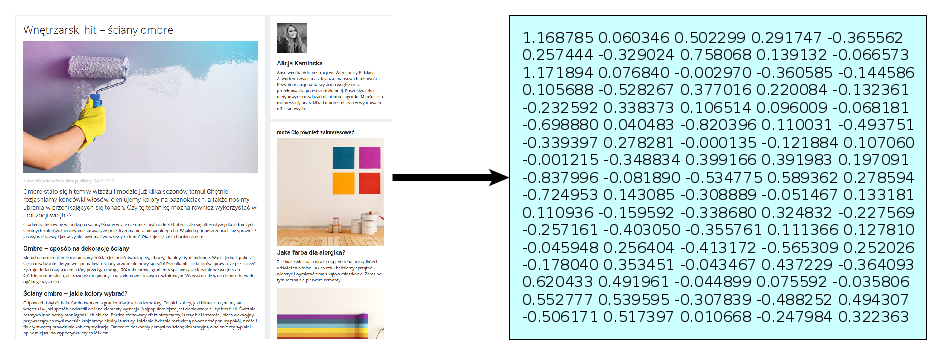
\includegraphics[width=0.85\textwidth]{img/approach_outline.png}
		\end{figure}
		\begin{figure}
			\centering
			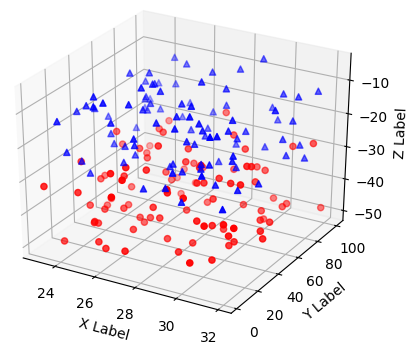
\includegraphics[width=0.45\textwidth]{img/scatter3d_demo.png}
		\end{figure}
	\end{frame}
	\note{
		\begin{itemize}
			\item Staramy się dokonać reprezentacji dokumentu w postaci wektora
			\item Po to, aby wykorzystać zależności między wektorami, np. odległość
			\item różne reprezentacje mają różną jakość
				\item odległości można mierzyć albo jako odległość euklidesową
				\item albo bardziej popularny sposób to kosinus kąta pomiędzy wektorami
			\end{itemize}}
			
			
	\begin{frame}{Bag-of-words i TF-IDF}
		\begin{itemize}
			\setlength\itemsep{2em}
			\item Dokumenty jako wektory
			\item Prostota implementacji
			\item Długie, niemalże ortogonalne wektory
			\item Brak informacji o kolejności słów
		\end{itemize}
	\end{frame}
	\note{\begin{itemize}
			\item korpus to zbiór dokumentów, na których operujemy
			\item słownik to lista unikalnych słów
			\item najprostsze podejście --- worek słów
			\item dokument jako wektor z liczbą wystąpień i-tego słowa na itym miejscu
			\item .
			\item Wadą jest traktowanie każdego słowa z~jednakową wagą
			\item bardzo długie wektory
			\item wektory niemalże ortogonalne
			\item prostota
			
			\item duża wymiarowość wektorów
			\item wektory niemalże ortogonalne
			
			\item zachowuje inne wady BOW
			\item bywa skłądową innych metod
		\end{itemize}}

	\begin{frame}{Latent semantic indexing (1988)}
		\begin{itemize}
			\setlength\itemsep{2em}
			\item ,,Słowa występujące w~tym samym kontekście niosą ze~sobą podobne znaczenie''
			\item Przyjmuje macierz wystąpień słów w~dokumentach
			\item Grupuje słowa w abstrakcyjne tematy
			\item Redukcja wymiarowości przez rozkład według wartości osobliwych
		\end{itemize}
			\begin{equation}
				A = U \Sigma V^T
			\end{equation}
	\end{frame}
	\note{\begin{itemize}
			\item kolejne metody opierają się na hipotezie, że słowa występujące w~tym samym kontekście niosą ze~sobą podobne znaczenie
			\item w LSI budujemy macierz wystąpień słów w dokumentach
			\item następnie wykonujemy redukcję liczby wierszy do liczby podanej jako hiperparametr
			\item macierz zachowuje powiązania między słowami 
			
			\item redukcja liczby wierszy za pomocą rozkładu wg. wartości osobliwych
			\item można potraktować jako grupowanie słów z odpowiednimi wagami
			\item ostatecznie zależnośic między dokumentami-wektorami są lepiej oddane
			\item wektory są krótkie
			\item jednak metoda ma nistą interpretowalność
		\end{itemize}}
	\begin{frame}{Latent Dirichlet allocation (2003)}
		\begin{itemize}
			\setlength\itemsep{2em}
			\item Automatyczne wykrywanie tematów zawartych w dokumentach
			\item Dokumenty jako mieszanki tematów
			\item Tematy jako rozkłady prawdopodobieństwa na zbiorze słów
			\item Początkowe przypisanie wg. rozkładu Dirichleta
			\item Iteracyjne poprawianie przypisań aż do stanu stabilnego
			\item Tematy łatwo interpretowalne
		\end{itemize}
	\end{frame}
	\note{\begin{itemize}
			\item Zadaniem metody jest reprezentacja dokumentów jako mieszanki tematów
			\item gdzie temat to mieszanka jawnych słów wybieranych z odpowiednimi wagami
			\item można to traktować jako redukcję wymiarowości
			\item liczba tematów określana hiperparametrem
			
			\item Początkowe przypisanie tematów do dokumentów i słów do tematów odbywa się zgodnie z rozkładem Dirichleta
			\item zaóżmy że mamy 3 tematy, którym odpowiadają wierznhołki trójkąta
			\item liczba dokumentów składających się z tylko jednego tematu jest niska
			\item liczba dokumentów składających się z mieszanki tematów jest wysoka
			\item .
			\item te cechy rozkładu Dirichleta przyspieszają optymalizację
		\item Rozkład daje pierwsze przybliżenie
		
		\item następnie iterujemy i przypisanie słów do tematów jest poprawiane
		
		\item dla każdego słowa w każdym dokumencie wyznaczany przypisywane jest temat, który jest najbardziej prawdopodobny na podstawie rozkładu w całości korpusu
		
		\item ostatecznie uzyskujemy w miarę stabilną sytuację, w której nie następują już zmiany przypisań słów do tematów
		
		\item podobne są dokumenty o podobnej proporcji przypisanych tematów
		
		\item metoda jest interpretowalne, gdyż wiemy, jakie słowa wchodzą w skłąd tematów
	\end{itemize}}
	\begin{frame}{Word embeddings}
		\begin{itemize}
			\item Osadzanie słów w przestrzeni wektorowej
			\item Uczenie nienadzorowane
			\item Niska wymiarowość wektorów
			\item Reprezentacja słów wraz z~zależnościami pomiędzy nimi
		\end{itemize}
		\begin{figure}
			\centering
			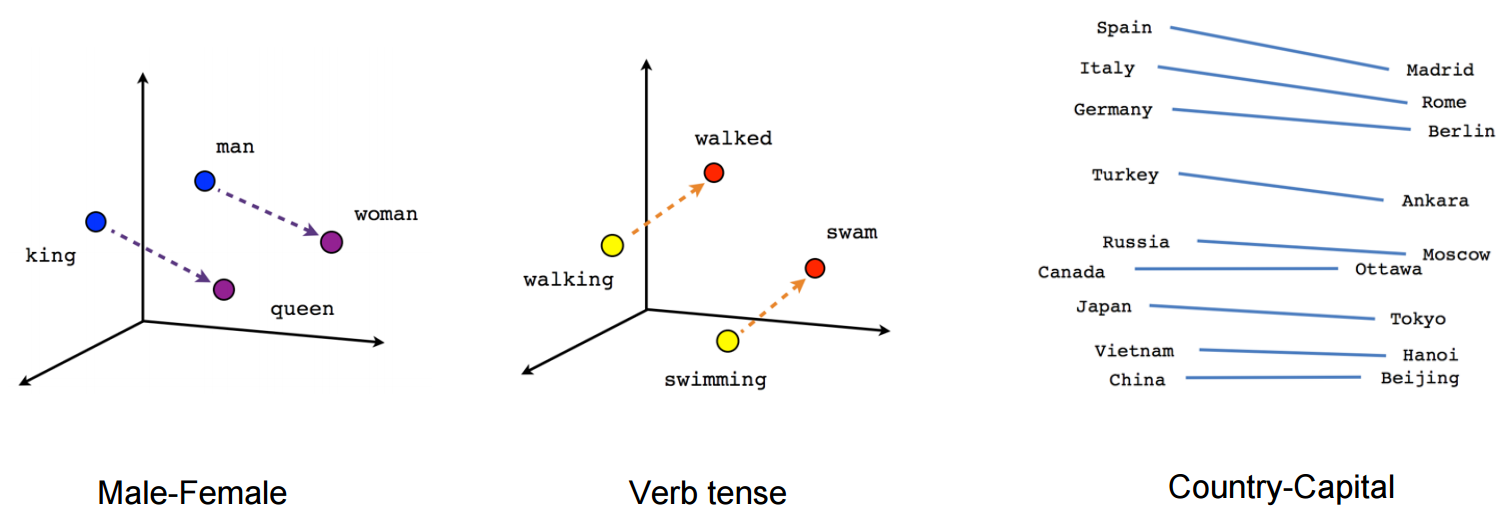
\includegraphics[width=1\textwidth]{img/linear-relationships.png}
		\end{figure}
		%https://www.tensorflow.org/images/linear-relationships.png
	\end{frame}
\note{\begin{itemize}
		\item Kolejnym podejściem jest osadzanie słów w przestrzeni wektorowej, a następnie porównywanie dokumentów jako list takich wektorów
		
		\item celem metod tej grupy jest przypisanie słowom takich wektorów, żeby zachowywały one zależności zachodzące między słowami
	\end{itemize}}

\begin{frame}{Word2vec (2013)}
	\begin{itemize}
		\setlength\itemsep{2em}
		\item Płytka sieć neuronowa feed-forward do predykcji słów
		\item Okno kontekstu skanujące korpus
		\item Predykcja słowa na podstawie jego kontekstu (bądź odwrotnie)
		\item Wyjściowe wektory zapisane w wagach warstwy ukrytej nauczonej sieci
		\item FastText (2016) --- rozwinięcie metody o analizę podsłów
	\end{itemize}
\end{frame}
\note{\begin{itemize}
		\item Kluczowym reprezentantem podejścia jest word2vec
		\item używa płytkiej sieci neuronowej feed-forward do predykcji słów
		\item .
		\item zbiór uczący jest skaowany oknem o zadanej wielkości
		słowa z każdego okna są wejćiem i wyjściem sieci wektorowej
		\item kodujemy je jeko one-hot-wektor czyli dla i-tego słowa wektor zer z jedynką n i-tym miejscu
		\item wyróżniamy dwa podejścia CBOW: predykcja słowa na podstawie konekstu
		\item skip-gram: predykcja kontekstu na podstawie słowa
		
		\item sieć zamiast funkcji aktywacji ma funkcję softmax, która zamienia wyjście na rozkłąd prawdopodobieństwa
		
		\item wektory reprezentujące słowa są efektem ubocznym nauczonej sieci
		\item zawarte są w wagach warstwy ukrytej i mają długość równą rozmiarowi tej warstwy
		
		\item wcześniejsze podejścia opierały się na głębszych sieciach, które działały mało wydajnie


		\item Jest modyfikacją word2vec
		\item powstało niedawno
		\item metoda rozbija słowo na n-gramy : podsłowa o określonej długości
		\item ostatecznie wektor słowa to suma wektoru słowa i wektorów podsłów
		\item sprawdza się dla języków bogatych morfosyntaktycznie
	\end{itemize}}
	\begin{frame}{GloVe --- Global Vectors (2014)}


\begin{enumerate}
	\setlength\itemsep{2em}
	\item Zgromadź współwystąpienia słów w formie globalnej macierzy $X$ takiej, że
	$X_{ij}$: ile razy słowo $i$ występuje w kontekście słowa $j$

	\item Zminimalizuj funkcję kosztu opartą na założeniu:
	\begin{equation}
	w_i^Tw_j \propto X_{ij},
	\end{equation}
	gdzie $w_i,\ w_j$ to wektorowe reprezentacje słów.
\end{enumerate}
	\end{frame}
\note{\begin{itemize}
		\item podejście alternatywne dla word2vec
		\item operuje na globalnej macierzy współwystąpień słow
		\item w funkcji celu najniższą wartość osiągniemy, gdy w1 * w2 będzie równe log(Xij) - jeżeli wektory są blisko siebie to iloczyn jest duży. jeżeli włowa są częstow w swoim kontekście to Xij jest duże.
		
		\item Celem funkcji optymalizacji funkcji kosztu jest minimalizacja różnicy pomiędzy iloczynami skalarnymi wektorów współwystępujących słów.
		
		\item wyniki podobne do word2vec
	\end{itemize}}
	\begin{frame}{Odległości między dokumentami word embeddings}
				\begin{itemize}
					\item centroid
							\begin{figure}
								\centering
								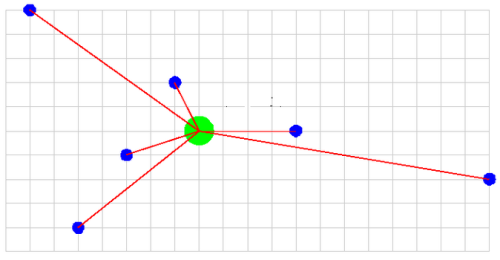
\includegraphics[width=0.5\textwidth]{img/centroid.png}
							\end{figure}
					\item Word Mover's Distance
							\begin{figure}
								\centering
								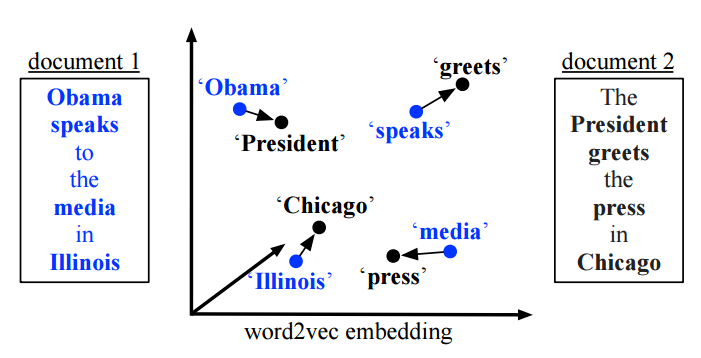
\includegraphics[width=0.5\textwidth]{img/wmd.png}
							\end{figure}
				\end{itemize}

	\end{frame}
\note{\begin{itemize}
		\item Mamy już wektorowe reprezentacje słów wchodzących w skład dokumentu - CO DALEJ
		\item można obliczyć średnią tych wektorów - centroid, ale przy tym traci się część informacji
		\item Alternatywą jest Word Mover's Distance
		\item Dystans pomiędzy dokumentami $A$ i $B$ to minimalny skumulowany dystans jaki słowa dokumentu $A$ muszą ,,przebyć'', aby osiągnąć słowa dokumnetu $B$
		\item Metoda jest kosztowna obliczeniowo
	\end{itemize}}
	\section{Analiza danych}
	\begin{frame}{Analiza danych}
		\begin{itemize}
			\setlength\itemsep{2em}
			\item 20000~artykułów tekstowych w~formacie \textit{JSON}
			\item język polski
			\item słowa specyficzne dla różnych branż
			% ,,hipertoniczny'', ,,autofocus''
			\item struktura artykułu:
			\begin{itemize}
				\item treść: tytuł, nagłówek, tekst
				\item metadane: id, kategoria, słowa kluczowe
			\end{itemize}
			% w pracy opisuję dokładne statystyki
		\end{itemize}
	\end{frame}
\note{\begin{itemize}
		\item 20000~artykułów tekstowych w~formacie \textit{JSON}
		\item język polski
		\item słowa specyficzne dla różnych branż
		% ,,hipertoniczny'', ,,autofocus''
		\item struktura artykułu:
		\begin{itemize}
			\item treść: tytuł, nagłówek, tekst
			\item metadane: id, kategoria, słowa kluczowe
		\end{itemize}
	\end{itemize}}

	\begin{frame}{Wstępne przetwarzanie}
		\begin{enumerate}
			\setlength\itemsep{2em}
			\item Oczyszczanie tekstu ze znaczników
			\item Usunięcie słów stopu
			\item Zamiana na małe litery
			\item Rozbicie słów połączonych myślnikiem
			\item Tokenizacja i lematyzacja % morfologik.blogspot.com
		\end{enumerate}
\note{\begin{itemize}
		\item w większości duże litery na początku zdania przeszkadzają, ale czasem wyraz z dużej litery i z małej znaczą co innego - Włochy
		\item lematyzacja to najistotniejszy element --- sprowadza słowa do postaci podstawowej
		\item np jest, była, będzie do ,,być''
		\item używam polskiego narzędzi Morfologik
	\end{itemize}}
	\end{frame}
	\begin{frame}{Preprocessing --- przykład}
		\begin{figure}
			\centering
			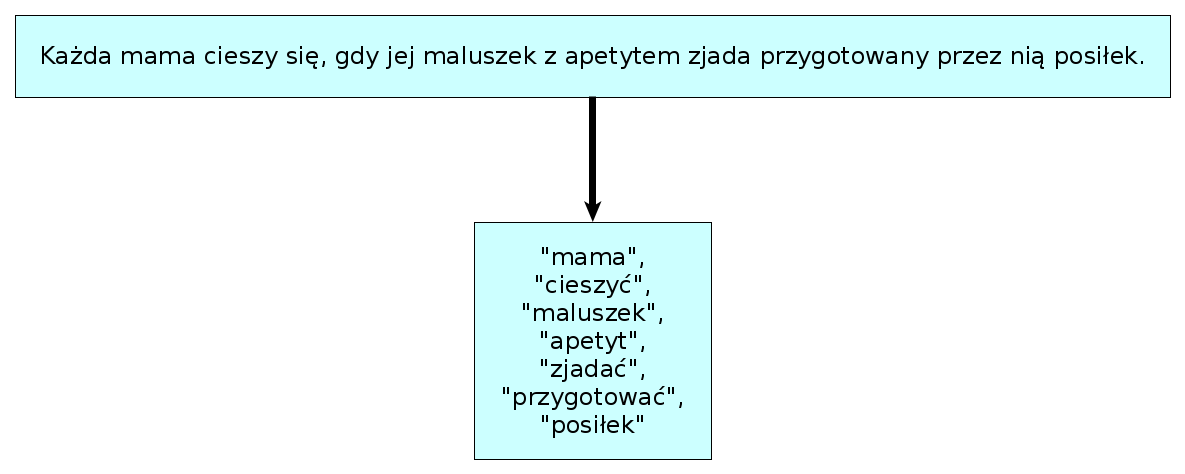
\includegraphics[width=1\textwidth]{img/lemmatisation.png}
		\end{figure}
	\end{frame}
	
\begin{frame}{Dane po przetworzeniu}
	\begin{itemize}
		\setlength\itemsep{2em}
		\item 7409145 tokenów, 98174 unikalnych
		\item Najczęstsze: ,,sam'', ,,uwaga'', ,,ważny'', ,,należeć'', ,,wybrać'', ,,sprawdzić'',
		,,model'', ,,miejsce'', ,,znaleźć''
		\item Najrzadsze: ,,naciągactwo'', ,,phone’ów'', ,,v90'',
		,,eurobusiness'', ,,namakać'', ,,bale’a'', ,,hmb'', ,,ameksyka'', ,,e-paper'', ,,süskind''
		\item Średnia długość artykułu: 370 słów
	\end{itemize}
\end{frame}
	% jaka byłaby sytuacja idealna? zaaplikować rozwiązania w żywym systemie i porównać kpi
	\section{Metody ewaluacji}
	
\note{\begin{itemize}
		\item W swojej pracy chcę sprawdzić, czy da się zastosować metody semantycznej analizy tekstu do generowania rekomendacji w allegro
		\item w tym celu dokonuję adaptacji opisanych wcześniej metod
		\item na wejściu daję artykuł i oczekuję listy rekomendacji
		\item .
		\item Pojęcie relewantności --- jak bardzo artykuł zarekomandowany jest związany z tym bazowym
		\item przykład: przepis na szarlotkę i oleje silnikowe są mało relewantne
	\end{itemize}}
	
	\begin{frame}{Miary jakości wyszukiwania}
		Zapytanie : ,,5 modeli frytownic na każdą kieszeń''
		\begin{figure}
			\centering
			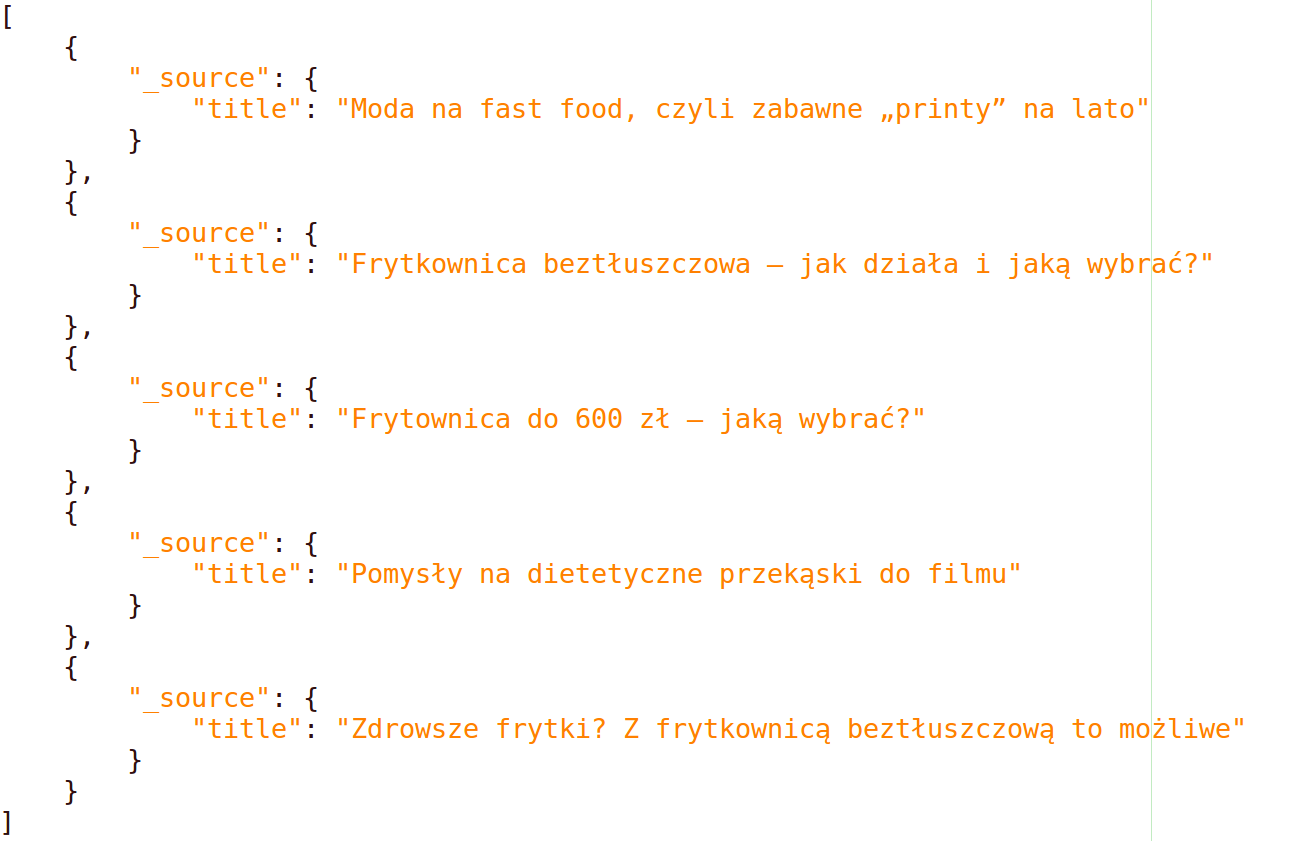
\includegraphics[width=0.7\textwidth]{img/elastic_result.png}
		\end{figure}
		
		\begin{itemize}
			\item Średnia relewantność
			\item NDCG: Normalized Discounted Cumulative Gain
		\end{itemize}
	\end{frame}
	\note{\begin{itemize}
			\item W celu oceny jakości rankingu można obliczyć jego średnią relewantność
			\item Albo można użyć miary DCG, która bierze pod uwagę kolejność wyników
			\item im bardziej relewantne wyniki, tym wyżej powinny być w~rankingu, aby ranking był najbardziej wartościowy

			\item Relewantność: W praktyce rzadko jednak dysponuje się wartością, na ile dany element rankingu jest adekwatny do zapytania generującego ów ranking.
		\end{itemize}}
	
	\begin{frame}{Miary relewantności}
		\begin{itemize}
			\setlength\itemsep{2em}
			\item Oparte na metadanych
			\begin{itemize}
				\item Liczba wspólnych kategorii
				\item Liczba wspólnych słów kluczowych
			\end{itemize}
			\item Oparte o historyczną aktywność użytkowników serwisu
			\item Ocena ekspercka użytkowników offline
		\end{itemize}

	\end{frame}
	\note{\begin{itemize}
			\item relewantność wyszukanych artykułów liczona na podstawie liczby wspólnych słów kluczowych z artykułem bazowym.
			\item Zaletą miar jest fakt, iż przypisanie artykułu do kategorii zostało wykonane przez autora, którego można określić ekspertem w dziedzinie tematyki artykułu
			\item można ją zastosować automatycznie
		\item Allegro zbiera w logach informację o kliknięciach użytkowników w linki
		\item skoro każdy artykuł posiada rekomendacje wygenerowane dotychczasową metodą to na podstawie liczby przejść na poszczególne rekomendacje można określić, która z nich jest najbardziej popularna
		\item tę popularność --- relewantność można zestawić z wynikami moich adaptacji metod 
			\item Do badania wygenerowałem każdą z wybranych metod rekomendacje do wylosowanych 50 artykułów
			\item podzieliłem je na pary artykuł bazowy --- artykuł rekomendowany
			\item zbudowałem lokalny interfejs webowy do ocenty tych par
			\item zaangażowałem 5 użytkowników, aby dokonali oceny, jak bardzo podobne są artykuły w poszczególnych parach
		\end{itemize}}
	\begin{frame}{Metodyka oceny eksperckiej}
		\begin{itemize}
			\setlength\itemsep{2em}
			\item Prosty interfejs webowy
			\item 5 użytkowników
			\item 50 artykułów bazowych, po 6 artykułów rekomendowanych
			\item Zbiór par testowych: artykuł bazowy --- artykuł rekomendowany
			\item Ocena testowanej metody: średnia ważona relewantność
		\end{itemize}
		
	\end{frame}
	\section{Wyniki testów}
\note{\begin{itemize}
		\item Ostatecznie testuję wybrane metody w zależności od ich hiperparametrów
		\item do ewaluacji stosuję opisane miary
		\item wszystkie wyniki są znormalizowane względem najlepszego wyniku w danym teście
	\end{itemize}}
	\begin{frame}{Zestawienie wyników}
		\begin{figure}[H]
			\centering
			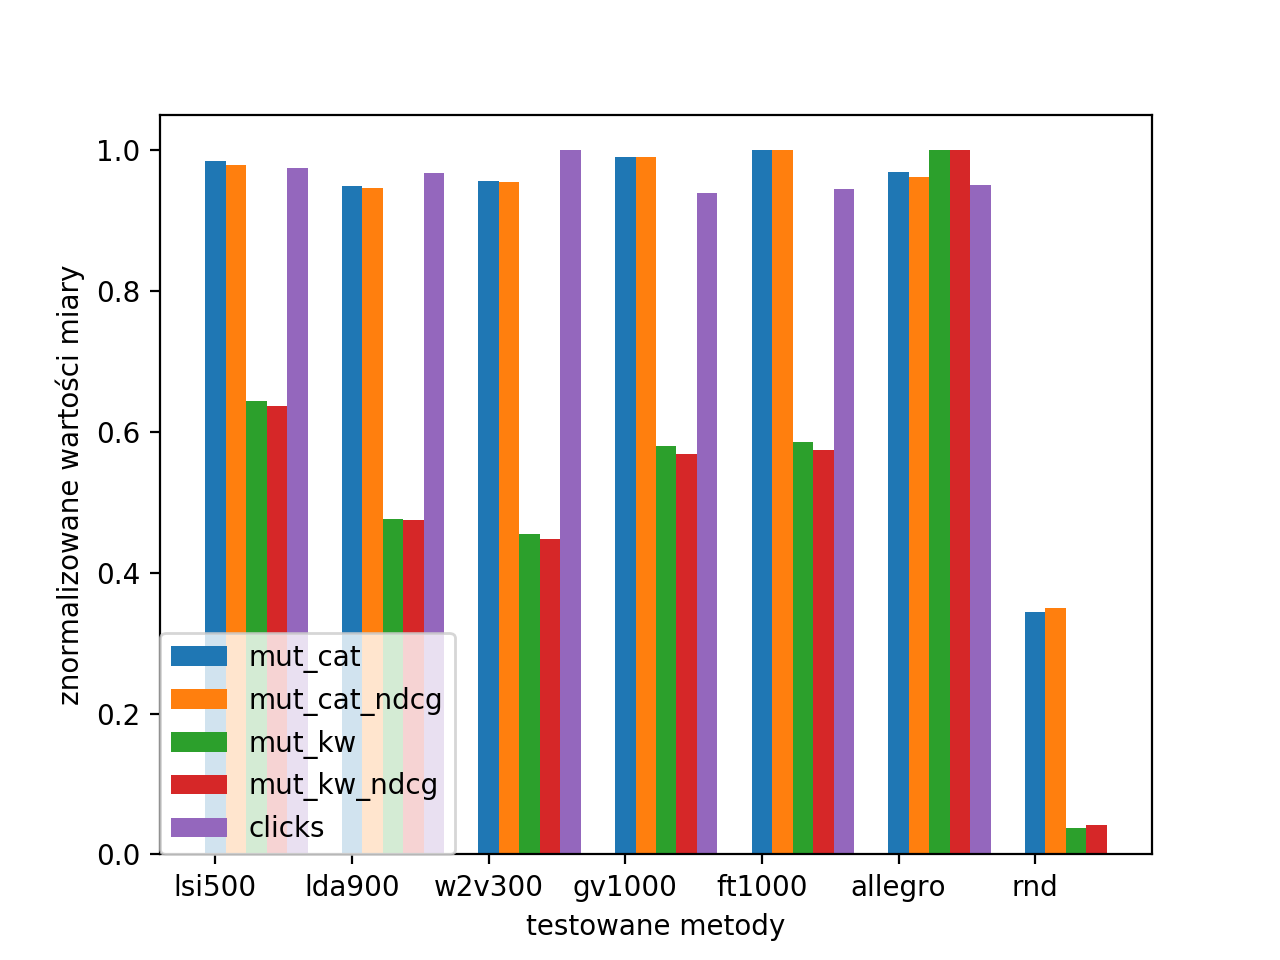
\includegraphics[width=1\textwidth]{img/results/lsi500_lda900_w2v300_gv1000_ft1000_allegro_rnd_.png}
		\end{figure}
	\end{frame}
	\begin{frame}{Wyniki ewaluacji eksperckiej dla~wybranych metod}
		\begin{figure}[H]
			\centering
			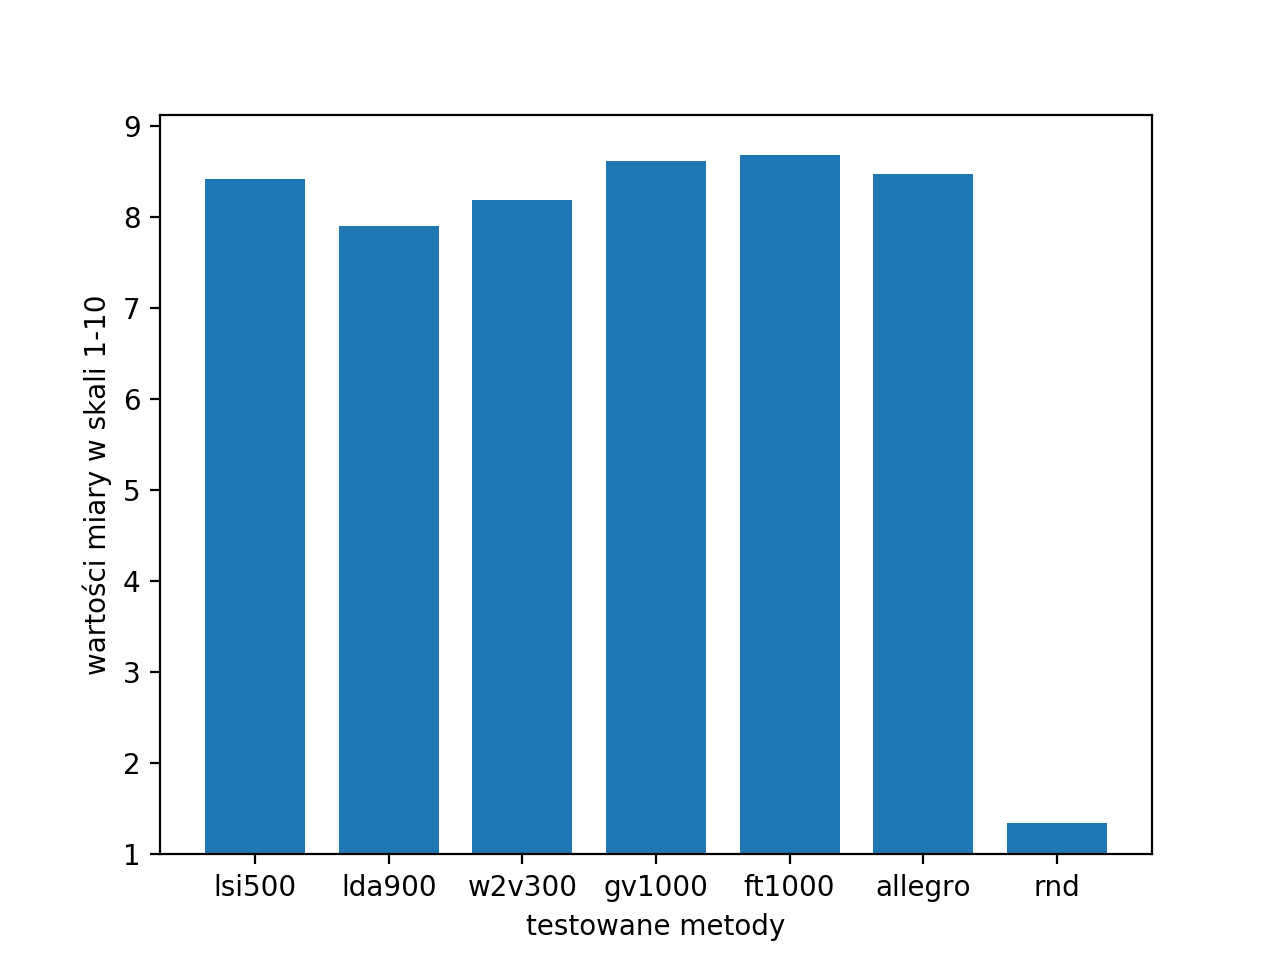
\includegraphics[width=0.8\textwidth]{img/results/lsi500_lda900_w2v300_gv1000_ft1000_allegro_rnd_users.png}
		\end{figure}
	\end{frame}
	\begin{frame}{Porównanie wyników ewaluacji eksperckiej metod}
		\begin{itemize}
			\setlength\itemsep{2em}
			\item Test Kruskala-Wallisa
			\item Średnia ocena użytkowników dla pierwszej rekomendacji do każdego z testowanych artykułów bazowych
			\item Nie ma podstaw, by sądzić, że wyniki metod różnią się w sposób statystycznie istotny
		\end{itemize}
	\end{frame}
	\section{Podsumowanie}
	\begin{frame}{Podsumowanie}
		\begin{itemize}
			\setlength\itemsep{1.1em}
			\item Brak istotnych statystycznie różnic między wynikami wszystkich metod
			\item Im dłuższe wektory \emph{word embeddings}, tym lepsze rezultaty
			\item Większa liczba tematów nie implikuje lepszych rezultatów
		\end{itemize}
		\begin{itemize}
			\setlength\itemsep{1.1em}
			\item Ewaluacja jest zadaniem nietrywialnym
			\item Szybki rozwój dziedziny
			\item Wiele kierunków dalszych badań
		\end{itemize}
	\end{frame}
\note{\begin{itemize}
		\item metoda oparta o kliknięcia okazała się słaba

		\item inne sposoby preprocesingu
		\item inne hiperparametry
		\item inne metody porównywania dokumentów - np testy A/B
	\end{itemize}}
	\section{Wybrane źródła}
	\begin{frame}{Wybrane źródła}
		\begin{thebibliography}{30}
			\bibitem{lda}
				D. M. Blei, A. Y. Ng, M. I. Jordan,
				\emph{Latent Dirichlet Allocation},
				Journal of Machine Learning Research, tom 3 num. 4–5,
				2003
			\bibitem{lsa}
				S. Deerwester, S. T. Dumais, G. W. Furnas, T. K. Landauer, R. Harshman,
				\emph{Indexing by latent semantic analysis},
				Journal of the American Society for Information Science, tom 41, num. 6,
				1990
			\bibitem{fasttext}
				A. Joulin, E. Grave, P. Bojanowski T. Mikolov,
				\emph{Bag of Tricks for Efficient Text Classification},
				Facebook AI Research,
				2016
			\bibitem{word2vec}
				T. Mikolov, K. Chen, G. Corrado, J. Dean,
				\emph{Efficient Estimation of Word Representations in Vector Space},
				International Conference on Machine Learning (ICML),
				2013
			\bibitem{glove}
				J. Pennington, R. Socher, C. D. Manning,
				\emph{GloVe: Global Vectors for Word Representation},
				Computer Science Department, Stanford University, Stanford, CA 94305,
				2014
		\end{thebibliography}
	\end{frame}
	\begin{frame}{}
		Dziękuję za uwagę
	\end{frame}
\end{document}
